\section{Preliminaries}\label{sec:preliminaries}

\noindent
\textbf{Model.}
We consider a setting where the blockchain network consists of two different
types of nodes: The first kind, \emph{full nodes}, are responsible for the
maintenance of the chain including verifying it and mining new blocks. The
second kind, \emph{verifiers} connect to full nodes and wish to learn facts
about the blockchain without downloading it, for example whether a particular
transaction is confirmed. The full nodes therefore also function as
\emph{provers} for the verifiers. Each verifier connects to multiple provers, at
least one of which is assumed to be honest.

We model full nodes according to the Backbone model~\cite{backbone}. There are
$n$ full nodes, of which $t$ are adversarial and $n - t$ are honest. All $t$
adversarial parties are controlled by one colluding adversary $\mathcal{A}$. The
parties have access to a hash function $H$ which is modelled as a common Random
Oracle~\cite{ro}. To each novel query, the random oracle outputs $\kappa$ bits
of fresh randomness. Time is split into distinct \emph{rounds} numbered by the
integers $1, 2, \cdots$. Our treatment is in the \emph{synchronous model}, so we
assume messages \emph{diffused} (broadcast) by an honest party at the end of a
round are received by all honest parties at the beginning of the next round.
This is equivalent to a network connectivity assumption in which the round
duration is taken to be the known time needed for a message to cross the
diameter of the network. The adversary can inject messages, reorder them, sybil
attack by creating multiple messages, but not suppress messages.

\noindent
\textbf{Blockchain.} Each honest full node locally maintains a \emph{chain} $\chain$, a sequence of
blocks. In understanding that we are developing an improvement on top of SPV, we
use the term \emph{block} to mean what is typically referred to as a
\emph{block header}. Each block contains the Merkle Tree root~\cite{merkle} of
transaction data $\overline{x}$, the hash $s$ of the previous block in the chain
known as the \emph{previd}, as well as a nonce value $ctr$. As discussed in the
Introduction, the compression of application data $\overline{x}$ is orthogonal
to our goals in this paper and has been explored in independent
work~\cite{edrax} which can be composed with ours. Each block $b = s \conc
\overline{x} \conc ctr$ must satisfy the proof-of-work~\cite{pow} equation $H(b) \leq T$
where $T$ is a constant \emph{target}, a small value signifying the difficulty
of the proof-of-work problem. Our treatment is in the \emph{static difficulty}
case, so we assume that $T$ is constant throughout the execution\footnote{A
treatment of variable difficulty NIPoPoWs has been explored in the soft fork
case~\cite{dionyziz}, but we leave the treatment of velvet fork NIPoPoWs in the
variable difficulty model for future work.}. $H(B)$ is
known as the \emph{block id}.

Blockchains are finite block sequences obeying the \emph{blockchain property}:
that in every block in the chain there exists a pointer to its previous block. A
chain is \emph{anchored} if its first block is \emph{genesis}, denoted $\mathcal{G}$,
a special block known to all parties. This is the only node the verifier knows about
when it boots up. For chain addressing we use Python brackets $\chain[\cdot]$. A
zero-based positive number in a bracket indicates the indexed block in the
chain. A negative index indicates a block from the end, e.g., $\chain[-1]$ is
the tip of the blockchain. A range $\chain[i{:}j]$ is a subarray starting from
$i$ (inclusive) to j (exclusive). Given chains $\chain_1, \chain_2$ and blocks
$A, Z$ we concatenate them as $\chain_1 \chain_2$ or $\chain_1 A$ (if clarity
mandates it, we also use the symbol $\conc$ for concatenation). Here,
$\chain_2[0]$ must point to $\chain_1[-1]$ and $A$ must point to $\chain_1[-1]$.
We denote $\chain\{A{:}Z\}$ the subarray of the chain from block $A$ (inclusive) to
block $Z$ (exclusive). We can omit blocks or indices from either side of the range to
take the chain to the beginning or end respectively. As long as the blockchain
property is maintained, we freely use the set operators $\cup$, $\cap$ and
$\subseteq$ to denote operations between chains, implying that the appropriate
blocks are selected and then placed in chronological order.

During every round, every party attempts to \emph{mine} a new block on top of
its currently adopted chain. Each party is given $q$ queries to the random
oracle which it uses in attempting to mine a new block. Therefore the adversary
has $tq$ queries per round while the honest parties have $(n - t)q$ queries per
round. When an honest party discovers a new block, they extend their chain with
it and broadcast the new chain. Upon receiving a new chain $\chain'$ from the
network, an honest party compares its length $|\chain'|$ against its currently
adopted chain $\chain$ and adopts the newly received chain if it is longer. It
is assumed that the honest parties control the majority of the computational
power of the network. This \emph{honest majority assumption} states that there
is some $\delta$ such that $t < (1 -  \delta)(n - t)$. If so, the protocol
ensures consensus among the honest parties: There is a constant $k$, the
\emph{Common Prefix} parameter, such that, at any round, all the chains
belonging to honest parties share a common prefix of blocks; the chains can
deviate only up to $k$ blocks at the end of each chain~\cite{backbone}.
Concretely, if at some round $r$ two honest parties have $\chain_1$ and
$\chain_2$ respectively, then either $\chain_1[{:}-k]$ is a prefix of $\chain_2$
or vice versa.

\noindent
\textbf{Superblocks.}
Some valid blocks satisfy the proof-of-work equation better than required. If
a block $b$ satisfies $H(b) \leq 2^{-\mu} T$ for some natural number
$\mu \in \mathbb{N}$ we say that $b$ is a \emph{$\mu$-superblock} or a block
\emph{of level} $\mu$. The probability of a new valid block achieving level
$\mu$ is $2^{-\mu}$. The number of levels in the chain will be $\log|\chain|$
with high probability~\cite{popow}. Given a chain $\chain$, we denote
$\chain\upchain^\mu$ the subset of $\mu$-superblocks of $\chain$.

Non-Interactive Proofs of Proof-of-Work (NIPoPoW) protocols allow verifiers to
learn the most recent $k$ blocks of the blockchain adopted by an honest full
node without downloading the whole chain. The challenge lies in building a
verifier who can find the suffix of the longest chain between claims of both
honest and adversarial provers, while not downloading all block headers. Towards
that goal, the \emph{superblock} approach uses superblocks as samples of
proof-of-work. The prover sends superblocks to the verifier to convince them
that proof-of-work has taken place without actually presenting all this
proof-of-work. The protocol is parametrized by a constant security parameter
$m$. The parameter determines how many superblocks will be sent by the prover to
the verifier and security is proven with overwhelming probability in $m$.

\noindent
\textbf{Prover.}
The prover selects various levels $\mu$ and for each such level sends a
carefully chosen portion of its $\mu$-level \emph{superchain}
$\chain\upchain^\mu$ to the verifier. In standard blockchain protocols such as
Bitcoin and Ethereum, each block $\chain[i + 1]$ in $\chain$ points to its
previous block $\chain[i]$, but each $\mu$-superblock $\chain\upchain^\mu[i +
1]$ does not point to its previous $\mu$-superblock $\chain\upchain^\mu[i]$. It
is imperative that an adversarial prover does not reorder the blocks within a
superchain, but the verifier cannot verify this unless each $\mu$-superblock
points to its most recently preceding $\mu$-superblock. The proposal is
therefore to \emph{interlink} the chain by having each $\mu$-superblock include
an extra pointer to its most recently preceding $\mu$-superblock. To ensure
integrity, this pointer must be included in the block header and verified by
proof-of-work. However, the miner does not know which level a candidate block
will attain prior to mining it. For this purpose, each block is proposed to
include a pointer to the most recently preceding $\mu$-superblock, for every
$\mu$, as illustrated in Figure~\ref{fig.hierarchy}. As these levels are only
$\log|\chain|$, this only adds $\log|\chain|$ extra pointers to each block
header.
\begin{algorithm}
    \caption{\label{alg.nipopow-prover}The \textsf{Prove} algorithm
    for the NIPoPoW protocol in a soft fork}
    \begin{algorithmic}[1]
        \Function{\sf Prove$_{m,k}$}{$\chain$}
            \Let{B}{\chain[0]}
            \Comment{Genesis}
            \For{$\mu = |\chain[-k-1].\mathsf{interlink}|$ down to $0$}
                \Let{\alpha}{\chain[:-k]\{B:\}\upchain^\mu}
                \Let{\pi}{\pi \cup \alpha}
                \If{$m < |\alpha|$}
                    \Let{B}{\alpha[-m]}
                \EndIf
            \EndFor
            \Let{\chi}{\chain[-k:]}
            \State\Return{$\pi\chi$}
        \EndFunction
    \vskip8pt
    \end{algorithmic}
\end{algorithm}


% \begin{figure}[ht]
%     \centering
%     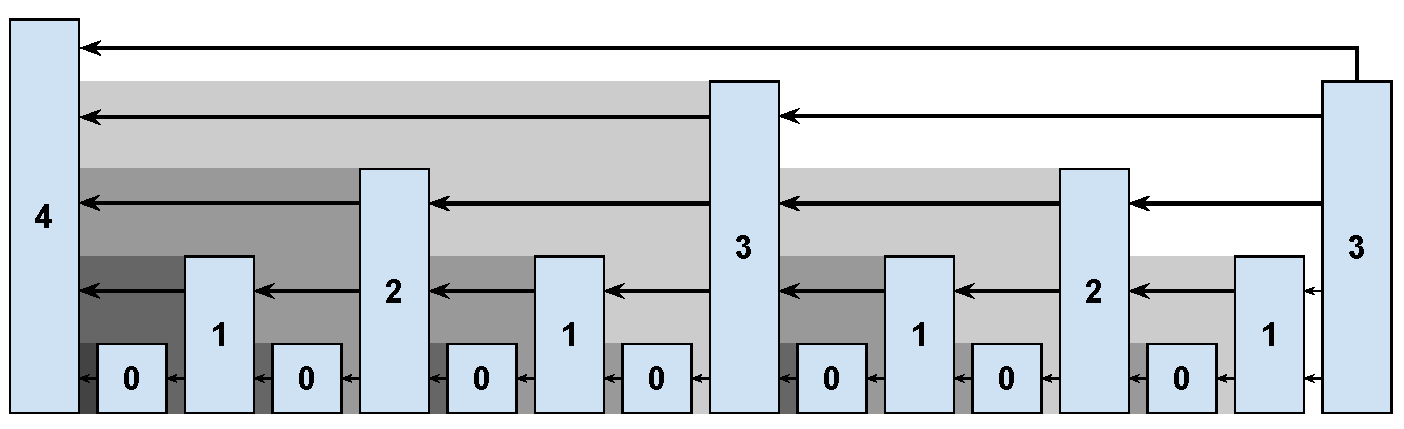
\includegraphics[width=0.9\columnwidth,keepaspectratio]{figures/prelims/level-shadows.pdf}
%     \caption{The interlinked blockchain. Each superblock is drawn taller
%     according to its achieved level. Each block links to all the blocks that are
%     not being overshadowed by their descendants. The most recent (right-most)
%     block links to the four blocks it has direct line-of-sight to.}
%     \label{fig.hierarchy}
% \end{figure}

The exact NIPoPoW protocol works like this: The prover holds a full chain
$\chain$. When the verifier requests a proof, the prover sends the last $k$
blocks of their chain, the suffix $\chi = \chain[-k{:}]$, in full. From the
larger prefix $\chain[{:}-k]$, the prover constructs a proof $\pi$ by selecting
certain superblocks as representative samples of the proof-of-work that took
place. The blocks are picked as follows. The prover selects the \emph{highest}
level $\mu^*$ that has at least $m$ blocks in it and includes all these blocks
in their proof (if no such level exists, the chain is small and can be sent in
full). The prover then iterates from level $\mu = \mu^* - 1$ down to $0$. For
every level $\mu$, it includes sufficient $\mu$-superblocks to cover the last
$m$ blocks of level $\mu + 1$, as illustrated in
Algorithm~\ref{alg.nipopow-prover}. Because the density of blocks doubles as
levels are descended, the proof will contain in expectation $2m$ blocks for each
level below $\mu^*$. As such, the total proof size $\pi \chi$ will be
$\Theta(m\log|\chain| + k)$. Such proofs that are polylogarithmic in the chain
size constitute an exponential improvement over traditional SPV clients and are
called \emph{succinct}.

\noindent \textbf{Verifier.} Upon receiving two proofs $\pi_1\chi_1,
\pi_2\chi_2$ of this form, the NIPoPoW verifier first checks that $\lvert
\chi_1 \rvert = \lvert \chi_2 \rvert = k$ and that $\pi_1 \chi_1$ and $\pi_2
\chi_2$ form valid chains. To check that they are valid chains, the verifier
ensures every block in the proof contains a pointer to its previous block
inside the proof through either the \emph{previd} pointer in the block header,
or in the interlink vector. If any of these checks fail, the proof is rejected.
It then compares $\pi_1$ against $\pi_2$ using the $\leq_m$ operator, which
works as follows. It finds the lowest common ancestor block $b = (\pi_1 \cap
\pi_2)[-1]$; that is, $b$ is the most recent block shared among the two proofs.
Subsequently, it chooses the level $\mu_1$ for $\pi_1$ such that $\lvert
\pi_1\{b{:}\}\upchain^{\mu_1} \rvert \geq m$ (i.e., $\pi_1$ has at least $m$
superblocks of level $\mu_1$ following block $b$) and the value $2^{\mu_1}
\lvert \pi_1\{b{:}\}\upchain^{\mu_1} \rvert$ is maximized.  It chooses a level
$\mu_2$ for $\pi_2$ in the same fashion. The two proofs are compared by
checking whether $2^{\mu_1} \lvert \pi_1\{b{:}\}\upchain^{\mu_1} \rvert \geq
2^{\mu_2} \lvert \pi_2\{b{:}\}\upchain^{\mu_2} \rvert$ and the proof with the
largest score is deemed the winner. The comparison is illustrated in
Algorithm~\ref{alg.nipopow-verifier}.

\begin{algorithm}[H]
    \caption{\label{alg.nipopow-verifier}The \textsf{Verify} algorithm
    for the NIPoPoW protocol}
    \begin{algorithmic}[1]
        \Function{{\sf best-arg}$_m$}{$\pi, b$}
            \Let{M}{\{\mu: |\pi\upchain^\mu\{b:\}| \geq m\} \cup \{0\}}
            \Comment{Valid levels}
            \State\Return{$\max_{\mu \in M}\{2^\mu  \cdot |\pi\upchain^\mu\{b:\}|\}$}
            \Comment{Score for level}
        \EndFunction
        \Operator{$\pi_A \geq_m \pi_B$}
            \Let{b}{(\pi_A \cap \pi_B)[-1]}
              \Comment LCA
            \State\Return{$\textsf{best-arg}_m(\pi_A, b) \geq
                           \textsf{best-arg}_m(\pi_B, b)$}
        \EndOperator
        \Function{\sf Verify$^Q_{m,k}$}{$\mathcal{P}$}
            \Let{\tilde\pi}{(\text{Gen})}
              \Comment{Trivial anchored blockchain}
            \For{$(\pi, \chi) \in \mathcal{P}$}
                \Comment{Examine each proof in $\mathcal{P}$}
                \If{$\mathsf{validChain}(\pi \chi)
                    \land |\chi| = k
                    \land \pi \geq_m \tilde\pi$}
                    \State{$\tilde\pi \gets \pi$}
                    \State{$\tilde\chi \gets \chi$}
                    \Comment{Update current best}
                \EndIf
            \EndFor
            \State\Return{$\tilde{Q}(\tilde\chi)$}
        \EndFunction
    \vskip8pt
    \end{algorithmic}
\end{algorithm}


\begin{algorithm}
    \caption{\label{alg.nipopow-verifier-infix}The \textsf{verify} algorithm
    for the NIPoPoW infix protocol}
    \begin{algorithmic}[1]
        \Function{\sf ancestors}{$B, \textsf{blockById}$}
            \If{$B = \text{Gen}$}
                \State\Return{$\{B\}$}
            \EndIf
            \Let{\chain}{\emptyset}
            \For{$\textsf{id} \in B.\textsf{interlink}$}
                \If{$\textsf{id} \in \textsf{blockById}$}
                    \Let{B'}{\textsf{blockById}[\textsf{id}]}
                    \Comment{Collect into DAG}
                    \Let{\chain}{\chain \cup \textsf{ancestors}(B', \textsf{blockById})}
                \EndIf
            \EndFor
            \State\Return{$\chain \cup \{B\}$}
        \EndFunction
        \Function{\sf verify-infx$^D_{\ell,m,k}$}{$\mathcal{P}$}
            \Let{\textsf{blockById}}{\emptyset}
            \For{$(\pi, \chi) \in \mathcal{P}$}
                \For{$B \in \pi$}
                    \Let{\textsf{blockById}[\textsf{id}(B)]}{B}
                \EndFor
            \EndFor
            \Let{\tilde\pi}{\text{best }\pi\in\mathcal{P}\text{ according to suffix verifier}}
            \State\Return{$D(\textsf{ancestors}(\tilde\pi[-1],
            \textsf{blockById}))$}
        \EndFunction
    \vskip8pt
    \end{algorithmic}
\end{algorithm}


In the case of the infix proofs there are some additional things that need to
be considered. An adversary prover could skip the blocks of interest and
present an honest and longer chain that, if only the suffix verifier where to
be used, is considered a better proof. For that reason, the last step of the
algorithm in the suffix verifier is changed to not only store the best proof
but also combine the two proofs by including all of the ancestor blocks of the
losing proof. This is guaranteed to include the blocks of interest. The
resulting best proof is stored as a DAG(Directed Acyclic Graph), as in
Algorithm~\ref{alg.nipopow-verifier-infix}
